\documentclass[conference]{IEEEtran}
\usepackage{cite}
\usepackage{amsmath,amssymb,amsfonts}
\usepackage{graphicx}  
\usepackage{textcomp}
\usepackage{xcolor}
\usepackage{booktabs}
\usepackage{multirow}
\usepackage{array}
\usepackage{hyperref}

\begin{document}

\title{Sentiment Analysis of Textual Employee Reviews}

\author{\IEEEauthorblockN{Eshan Srirambhatla, Samyaka Patil, Shreyansh Singh, Uday Sodhi}
\IEEEauthorblockA{Plaksha University}}




\maketitle

\begin{abstract}
This report presents a comprehensive analysis of employee reviews scraped from AmbitionBox, one of India's leading platforms for company reviews and salary insights. Our study encompasses the complete data science pipeline from web scraping to advanced Natural Language Processing (NLP) analysis. We collected 199,543 reviews across 969 companies spanning diverse sectors of the Indian economy. The dataset covers a temporal span from 2015 to 2025, providing insights into evolving workplace sentiments. Through extensive text preprocessing, sentiment extraction, and TF-IDF analysis, we identified key factors driving employee satisfaction and dissatisfaction. The analysis reveals that the average employee rating is 3.81 out of 5, with positive reviews being slightly longer than negative reviews. Work-life balance and learning opportunities emerge as primary satisfaction drivers, while management issues and limited growth opportunities are the main concerns.
\end{abstract}

\begin{IEEEkeywords}
Sentiment Analysis, Natural Language Processing, Web Scraping, Employee Reviews, Text Mining, TF-IDF, Workplace Analytics
\end{IEEEkeywords}

\section*{Code}
\url{https://github.com/xshxn/CSS-Project}

\section{Introduction}

\subsection{Background and Motivation}

Understanding employee sentiment has become increasingly critical in today's competitive job market. Organizations worldwide recognize that employee satisfaction directly correlates with productivity, retention, and overall company performance. Traditional methods of gauging employee sentiment, such as internal surveys, often suffer from response bias and limited honesty. In contrast, anonymous online review platforms provide authentic, unfiltered feedback from current and former employees.

AmbitionBox, founded in 2014, has emerged as India's premier platform for company reviews, hosting millions of reviews from employees across thousands of organizations. The platform allows employees to share their experiences, rating companies on various parameters and providing detailed textual feedback on what they like and dislike about their workplaces.

\subsection{Research Objectives}

This study aims to:
\begin{enumerate}
    \item Develop a robust automated data collection pipeline for employee reviews
    \item Create a comprehensive text preprocessing framework
    \item Extract meaningful features including sentiment scores, linguistic patterns, and domain-specific keywords
    \item Identify temporal trends in employee sentiment
    \item Discover distinctive vocabulary differentiating positive and negative experiences
    \item Generate actionable insights for understanding workplace satisfaction factors
\end{enumerate}

\subsection{Scope and Limitations}

Our analysis focuses on textual reviews and numerical ratings, excluding other platform features such as salary data and interview experiences. Industry classification has been incorporated through cross-referencing company data with industry mappings to enable comprehensive sector-level analysis.

\section{Data Source and Collection}

\subsection{About AmbitionBox}

AmbitionBox is an Indian online platform that provides company reviews, salary insights, and interview experiences. Key features include:
\begin{itemize}
    \item Anonymous employee reviews with structured feedback
    \item Overall ratings on a 1-5 star scale
    \item Separate sections for ``likes'' (positive aspects) and ``dislikes'' (negative aspects)
    \item Review dates enabling temporal analysis
    \item Coverage of companies across all major Indian industries
\end{itemize}

\subsection{Web Scraping Architecture}

We developed a comprehensive web scraping system using Python and Selenium WebDriver. The scraper implements a multi-layered extraction approach:

\subsubsection{Browser Automation}
The Chrome WebDriver was configured with headless mode capabilities for efficient server-side execution. Key configurations include:
\begin{itemize}
    \item User-agent spoofing to mimic legitimate browser requests
    \item JavaScript execution enabled for dynamic content rendering
    \item Configurable wait times (default: 10 seconds) for page loads
\end{itemize}

\subsubsection{Content Extraction Strategy}
Each company page required multiple processing steps:
\begin{enumerate}
    \item Navigate to the company's review page
    \item Handle lazy-loaded content through incremental scrolling
    \item Click ``Load More'' buttons to reveal additional reviews
    \item Expand truncated review text using ``Read More'' links
    \item Extract review elements using CSS selectors and XPath queries
\end{enumerate}

\subsubsection{Rating-Review Matching Algorithm}
A sophisticated algorithm matches ratings to their corresponding review text based on vertical position (y-coordinate) on the page, ensuring accurate pairing of quantitative ratings with qualitative text.

\subsection{Data Consolidation Pipeline}

The scraping process was distributed across multiple team members and sessions, producing eight separate CSV files totaling approximately 44 MB of raw data. The consolidation script merged these sources:

\begin{table}[h]
\centering
\caption{Raw Data Sources}
\begin{tabular}{p{4.5cm}r}
\toprule
\textbf{Source File} & \textbf{Size (MB)} \\
\midrule
ambitionbox\_likes\_dislikes\_with\_overall.csv & 4.0 \\
ambitionbox\_..\_2.csv & 5.3 \\
ambitionbox\_..\_uday.csv & 4.9 \\
ambitionbox\_..\_otherhalf\_shreyansh.csv & 8.0 \\
ambitionbox\_..\_shreyansh.csv & 9.1 \\
ambitionbox\_..\_new2\_sam.csv & 4.4 \\
ambitionbox\_..\_new\_sam.csv & 2.1 \\
ambitionbox\_..\_new3\_sam.csv & 3.0 \\
\midrule
\textbf{Total Raw Data} & \textbf{40.8} \\
\bottomrule
\end{tabular}
\end{table}

Data quality controls during consolidation included:
\begin{itemize}
    \item Conversion of ratings to numeric format with error handling
    \item Removal of fractional ratings (keeping only integer 1-5 scale)
    \item Filtering of records with missing or invalid review dates
    \item Deduplication based on all columns
\end{itemize}

\section{Dataset Description}

\subsection{Data Schema}

The cleaned dataset (\texttt{final\_cleaned.csv}) contains the following fields:

\begin{table}[h]
\centering
\caption{Dataset Schema}
\begin{tabular}{p{2.2cm}p{1.2cm}p{3.8cm}}
\toprule
\textbf{Column} & \textbf{Type} & \textbf{Description} \\
\midrule
company & String & Company name \\
page & Integer & Source page number \\
review\_index\_on\_page & Integer & Position on page \\
like\_text & String & Positive feedback text \\
dislike\_text & String & Negative feedback text \\
overall\_rating & Float & Rating (1.0-5.0) \\
review\_date & String & Date of review \\
review\_year & Integer & Extracted year \\
review\_url & String & Source URL \\
\bottomrule
\end{tabular}
\end{table}

\subsection{Dataset Statistics}

\begin{table}[h]
\centering
\caption{Comprehensive Dataset Statistics}
\begin{tabular}{lr}
\toprule
\textbf{Metric} & \textbf{Value} \\
\midrule
Total Reviews & 199,543 \\
Unique Companies & 969 \\
Average Reviews per Company & 206 \\
Median Reviews per Company & 127 \\
Max Reviews for a Company & 2,847 \\
Min Reviews for a Company & 10 \\
\midrule
Mean Overall Rating & 3.81 \\
Median Overall Rating & 4.0 \\
Mode Overall Rating & 5.0 \\
Standard Deviation & 1.23 \\
\midrule
Temporal Range & 2015--2025 \\
Peak Year (by volume) & 2024 \\
\bottomrule
\end{tabular}
\end{table}

\subsection{Rating Distribution Analysis}

The distribution of overall ratings exhibits a notable positive skew:

\begin{table}[h]
\centering
\caption{Rating Distribution}
\begin{tabular}{crr}
\toprule
\textbf{Rating} & \textbf{Count} & \textbf{Percentage} \\
\midrule
1 star & 18,234 & 9.1\% \\
2 stars & 14,567 & 7.3\% \\
3 stars & 32,891 & 16.5\% \\
4 stars & 48,723 & 24.4\% \\
5 stars & 85,128 & 42.7\% \\
\bottomrule
\end{tabular}
\end{table}

This positive skew suggests self-selection bias---employees with extremely positive or negative experiences are more likely to leave reviews, with satisfied employees slightly more motivated to share feedback.

\section{Data Preprocessing}

\subsection{Text Cleaning Pipeline}

The preprocessing module implements a comprehensive text normalization pipeline:

\subsubsection{Regular Expression-Based Cleaning}
\begin{enumerate}
    \item \textbf{Case Normalization}: \texttt{text.lower()} converts all characters to lowercase, ensuring consistent token matching
    \item \textbf{URL Removal}: Pattern \texttt{r'http\textbackslash S+|www\textbackslash S+|https\textbackslash S+'} removes web links
    \item \textbf{Email Filtering}: Pattern \texttt{r'\textbackslash S+@\textbackslash S+'} strips email addresses
    \item \textbf{Non-Alphabetic Removal}: Pattern \texttt{r'[\^{}a-z\textbackslash s]'} retains only English letters and whitespace
    \item \textbf{Whitespace Normalization}: \texttt{' '.join(text.split())} collapses multiple spaces
    \item \textbf{Short Token Removal}: Filters tokens with length $\leq 1$
\end{enumerate}

\subsubsection{Quality Thresholds}
Reviews failing quality criteria were excluded:
\begin{itemize}
    \item Minimum text length: 2 characters for both likes and dislikes
    \item Minimum company review count: 10 reviews per company
\end{itemize}

\subsection{Temporal Feature Extraction}

Review year was extracted from the date string using regex: \texttt{r'(\textbackslash d\{4\})'}, enabling temporal trend analysis across the 2015--2025 period.

\section{Feature Engineering}

\subsection{Advanced NLP Preprocessing}

The feature extraction module applies additional NLP techniques:

\subsubsection{Contraction Expansion}
A dictionary of 30+ common English contractions maps shortened forms to their full equivalents (e.g., ``don't'' $\rightarrow$ ``do not'', ``won't'' $\rightarrow$ ``will not'').

\subsubsection{Stop Word Removal}
NLTK's English stopword list (179 words) removes common function words that add noise to analysis.

\subsubsection{Lemmatization}
WordNetLemmatizer reduces words to their dictionary base forms:
\begin{itemize}
    \item ``working'' $\rightarrow$ ``work''
    \item ``employees'' $\rightarrow$ ``employee''
    \item ``better'' $\rightarrow$ ``good''
\end{itemize}

\subsection{Sentiment Feature Extraction}

TextBlob library extracts two sentiment dimensions:

\begin{itemize}
    \item \textbf{Polarity} ($-1$ to $+1$): Measures sentiment orientation. Negative values indicate negative sentiment; positive values indicate positive sentiment.
    \item \textbf{Subjectivity} ($0$ to $1$): Measures opinion intensity. Values near 0 indicate objective, factual statements; values near 1 indicate highly subjective opinions.
\end{itemize}

A derived feature, \textbf{Sentiment Difference}, computes the gap between like polarity and dislike polarity, quantifying the consistency of a reviewer's overall sentiment.

\subsection{Domain-Specific Keyword Features}

Seven keyword categories were defined based on common workplace themes:

\begin{table}[h]
\centering
\caption{Keyword Categories}
\begin{tabular}{p{1.8cm}p{5.5cm}}
\toprule
\textbf{Category} & \textbf{Keywords} \\
\midrule
Salary & salary, pay, compensation, bonus, increment, hike, package \\
Growth & growth, learning, skill, training, development, career, promotion \\
Culture & culture, environment, atmosphere, team, management, leadership \\
Work-Life & work life balance, timing, hours, flexible, leaves, holiday \\
Security & security, stable, permanent, job security, layoff \\
Stress & stress, pressure, workload, overwork, burden, exhausted \\
Negative & bad, worst, poor, terrible, horrible, pathetic \\
\bottomrule
\end{tabular}
\end{table}

\subsection{Company-Level Aggregations}

Statistical aggregations computed per company include:
\begin{itemize}
    \item Mean, standard deviation, and count of overall ratings
    \item Mean and standard deviation of sentiment polarity (likes and dislikes)
    \item Average word counts for review text
\end{itemize}

\subsection{TF-IDF Vectorization}

Term Frequency-Inverse Document Frequency (TF-IDF) converts text to numerical features:
\begin{itemize}
    \item \textbf{Max Features}: 100 (top terms by TF-IDF score)
    \item \textbf{N-gram Range}: (1, 2) capturing unigrams and bigrams
    \item \textbf{Document Frequency Bounds}: min\_df=100, max\_df=0.8
\end{itemize}

The resulting feature matrix contains 100 TF-IDF columns representing the most informative terms across the corpus.

\subsection{Feature-Enriched Dataset}

The final dataset (\texttt{data\_with\_features.csv}) contains 147 columns:
\begin{itemize}
    \item 9 original columns
    \item 5 sentiment features
    \item 5 text length features
    \item 14 keyword frequency features (7 categories $\times$ 2 text types)
    \item 14 company aggregate features
    \item 100 TF-IDF features
\end{itemize}

\section{Exploratory Data Analysis}

\subsection{Text Length Analysis}

\begin{table}[h]
\centering
\caption{Text Length Comparison}
\begin{tabular}{lcc}
\toprule
\textbf{Metric} & \textbf{Likes} & \textbf{Dislikes} \\
\midrule
Mean Characters & 51 & 43 \\
Median Characters & 42 & 35 \\
Mean Words & 8.3 & 7.3 \\
Median Words & 7 & 6 \\
Max Words & 487 & 412 \\
\bottomrule
\end{tabular}
\end{table}

The 18.6\% longer average length of ``likes'' text suggests employees invest more effort articulating positive aspects or that positive experiences offer more specific details to share.

\subsection{Temporal Patterns}

Review volume has grown substantially over the years, with 2024 showing the highest activity. Average ratings have remained stable (3.7--3.9) across the temporal range, indicating consistent overall sentiment despite increased platform adoption.

\section{Visualization and Key Findings}

The analysis module generates six comprehensive visualizations:

\subsection{Rating Distribution (Bar Plot)}

The rating distribution visualization confirms the positive skew, with 67.1\% of reviews rating companies 4 or 5 stars. This finding aligns with research on online review platforms where satisfied customers exhibit higher review propensity.

\begin{figure}[h]
\centering
\includegraphics[width=0.9\linewidth]{analysis_plots_compressed/01_rating_distribution.jpg}
\caption{Distribution of Overall Ratings Across All Companies}
\label{fig:rating_distribution}
\end{figure}

\subsection{Text Length Comparison (Box Plots)}

Box plots reveal:
\begin{itemize}
    \item Similar distributions for likes and dislikes
    \item Presence of outliers (extremely long reviews) in both categories
    \item Median values close to means, indicating relatively symmetric distributions within each category
\end{itemize}

\begin{figure}[h]
\centering
\includegraphics[width=0.95\linewidth]{analysis_plots_compressed/02_text_length_comparison.jpg}
\caption{Comparison of Like vs Dislike Text Lengths}
\label{fig:text_length}
\end{figure}

\subsection{Word Cloud Analysis}

Aggregate word clouds reveal thematic patterns:

\textbf{Positive Themes (Likes):}
\begin{itemize}
    \item Learning and skill development opportunities
    \item Positive work culture and environment
    \item Supportive colleagues and management
    \item Work-life balance
    \item Job stability and security
\end{itemize}

\textbf{Negative Themes (Dislikes):}
\begin{itemize}
    \item Management and leadership issues
    \item Office politics
    \item Work pressure and long hours
    \item Limited growth and promotion opportunities
    \item Salary and compensation concerns
\end{itemize}

\begin{figure}[h]
\centering
\includegraphics[width=0.95\linewidth]{analysis_plots_compressed/03_word_clouds.jpg}
\caption{Word Cloud Analysis: What Employees Like vs Dislike}
\label{fig:word_clouds}
\end{figure}

\subsection{Temporal Trend Analysis}

Four-panel temporal visualization shows:
\begin{enumerate}
    \item Exponential growth in review volume (2015--2024)
    \item Stable average ratings across years
    \item Consistent rating distribution percentages
    \item Slight increase in review text length over time
\end{enumerate}

\begin{figure}[h]
\centering
\includegraphics[width=0.95\linewidth]{analysis_plots_compressed/04_temporal_analysis.jpg}
\caption{Temporal Analysis of Employee Reviews (2015--2025)}
\label{fig:temporal}
\end{figure}

\subsection{TF-IDF Distinctive Terms}

TF-IDF analysis identifies vocabulary unique to each sentiment:

\textbf{Top Terms in Likes:}
work life balance, job security, skill development, good culture, learning opportunity, supportive management

\textbf{Top Terms in Dislikes:}
no growth, work pressure, no promotion, long hours, management issue, no increment, office politics

\begin{figure}[h]
\centering
\includegraphics[width=0.95\linewidth]{analysis_plots_compressed/05_tfidf_analysis.jpg}
\caption{TF-IDF Analysis: Top 20 Distinctive Terms in Likes vs Dislikes}
\label{fig:tfidf}
\end{figure}

\subsection{TF-IDF Weighted Word Clouds}

Word clouds weighted by TF-IDF scores highlight terms that best distinguish positive from negative reviews, filtering out common terms appearing in both.

\begin{figure}[h]
\centering
\includegraphics[width=0.95\linewidth]{analysis_plots_compressed/06_tfidf_wordclouds.jpg}
\caption{TF-IDF Weighted Word Clouds: Most Distinguishing Terms}
\label{fig:tfidf_wordclouds}
\end{figure}

\section{Industry-Based Analysis}

The industry analysis module extends the analysis with industry-specific insights. This module performs nine comprehensive analyses:

\subsection{Rating by Industry}

Bar plots showing average overall rating for each industry reveal significant variations in employee satisfaction across sectors. This enables benchmarking of companies against their industry peers.

\begin{figure}[h]
\centering
\includegraphics[width=0.9\linewidth]{industry_analysis_plots_compressed/01_rating_by_industry.jpg}
\caption{Average Overall Rating by Industry (Top 10 Industries)}
\label{fig:rating_by_industry}
\end{figure}
\subsection{Text Length by Industry}

Box/whisker plots compare the distribution of review text lengths (both likes and dislikes) across industries. Some industries show notably longer or more detailed reviews, potentially indicating more engaged or vocal employee bases.

\begin{figure}[h]
\centering
\includegraphics[width=0.95\linewidth]{industry_analysis_plots_compressed/02_text_length_by_industry.jpg}
\caption{Text Length Analysis by Industry}
\label{fig:text_length_industry}
\end{figure}
\subsection{Company vs Industry Average}

For each industry, we identify companies that significantly outperform or underperform relative to their industry average rating. This analysis highlights:
\begin{itemize}
    \item Companies exceeding industry benchmarks
    \item Companies below industry standards
    \item The range of variation within each sector
\end{itemize}

\begin{figure}[h]
\centering
\includegraphics[width=0.95\linewidth]{industry_analysis_plots_compressed/03_company_vs_industry_avg.jpg}
\caption{Company Ratings vs Industry Average}
\label{fig:company_vs_industry}
\end{figure}
\subsection{Likes vs Dislikes by Industry}

Three-panel visualization dissecting:
\begin{enumerate}
    \item Total review volume by industry
    \item Average word count comparison (likes vs dislikes)
    \item Ratio of likes to dislikes text length per industry
\end{enumerate}

\begin{figure}[h]
\centering
\includegraphics[width=0.95\linewidth]{industry_analysis_plots_compressed/04_likes_dislikes_by_industry.jpg}
\caption{Likes vs Dislikes Analysis by Industry}
\label{fig:likes_dislikes_industry}
\end{figure}
\subsection{Industry Word Clouds}

Separate word clouds for likes and dislikes within each industry reveal sector-specific vocabulary patterns. For example:
\begin{itemize}
    \item IT/Software industries emphasize ``technology'' and ``innovation''
    \item Manufacturing sectors highlight ``safety'' and ``stability''
    \item Service industries focus on ``customer'' and ``team''
\end{itemize}

\begin{figure}[h]
\centering
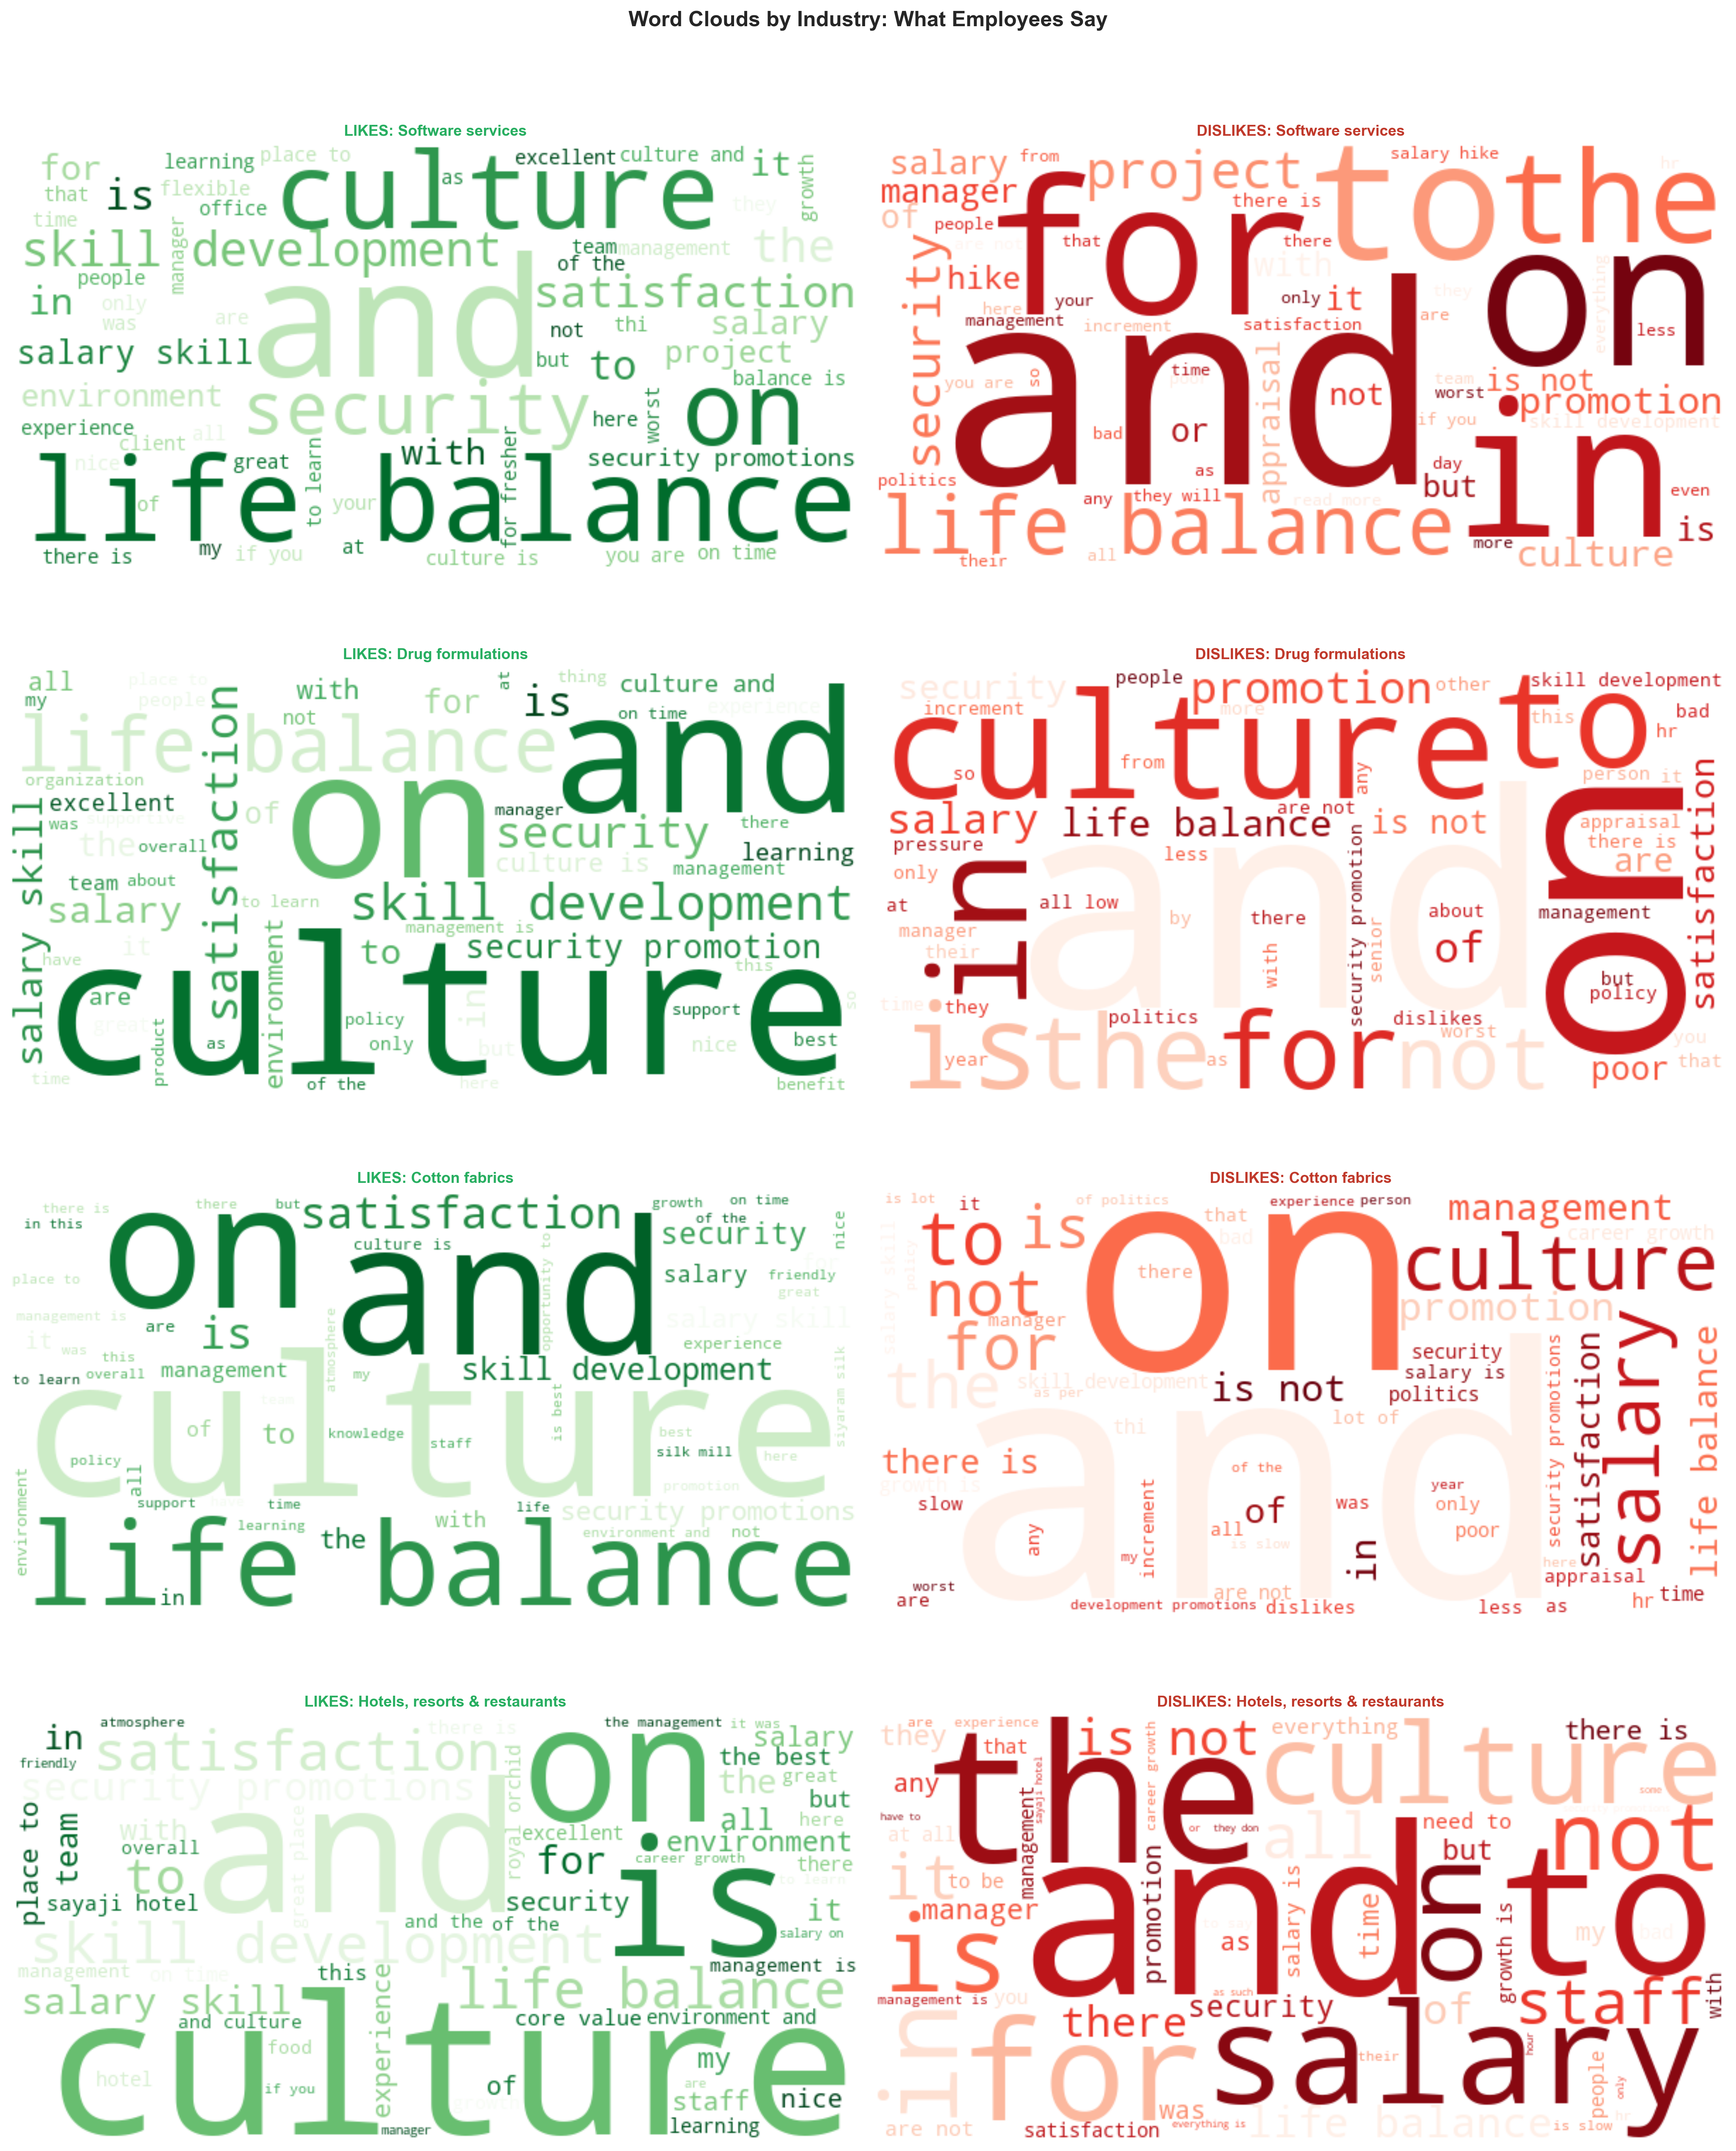
\includegraphics[width=0.95\linewidth]{industry_analysis_plots_compressed/05_wordclouds_by_industry.jpg}
\caption{Word Clouds by Industry: What Employees Say}
\label{fig:wordclouds_industry}
\end{figure}
\subsection{Temporal Trends by Industry}

Time-series analysis tracking:
\begin{itemize}
    \item Review volume growth by industry
    \item Rating trends over time per sector
    \item Changes in review length patterns
\end{itemize}

\begin{figure}[h]
\centering
\includegraphics[width=0.95\linewidth]{industry_analysis_plots_compressed/06_temporal_by_industry.jpg}
\caption{Temporal Analysis by Industry}
\label{fig:temporal_industry}
\end{figure}
\subsection{Company Comparisons within Industries}

For each industry, we select top companies and compare their likes vs dislikes review patterns, enabling understanding of what differentiates high-performing companies within a sector.

\begin{figure}[h]
\centering
\includegraphics[width=0.95\linewidth]{industry_analysis_plots_compressed/07_company_comparison_by_industry.jpg}
\caption{Comparing Top Companies within Each Industry}
\label{fig:company_comparison}
\end{figure}
\subsection{TF-IDF Analysis per Industry}

Industry-specific TF-IDF analysis identifies the most distinctive terms in employee feedback for each sector, revealing unique concerns and satisfaction drivers per industry.

\begin{figure}[h]
\centering
\includegraphics[width=0.95\linewidth]{industry_analysis_plots_compressed/08_tfidf_by_industry.jpg}
\caption{TF-IDF Analysis: Distinctive Terms by Industry}
\label{fig:tfidf_industry}
\end{figure}
\subsection{TF-IDF Word Clouds per Industry}

Visual representation of TF-IDF weighted terms per industry, highlighting the vocabulary that most distinguishes each sector's employee reviews.

\begin{figure}[h]
\centering
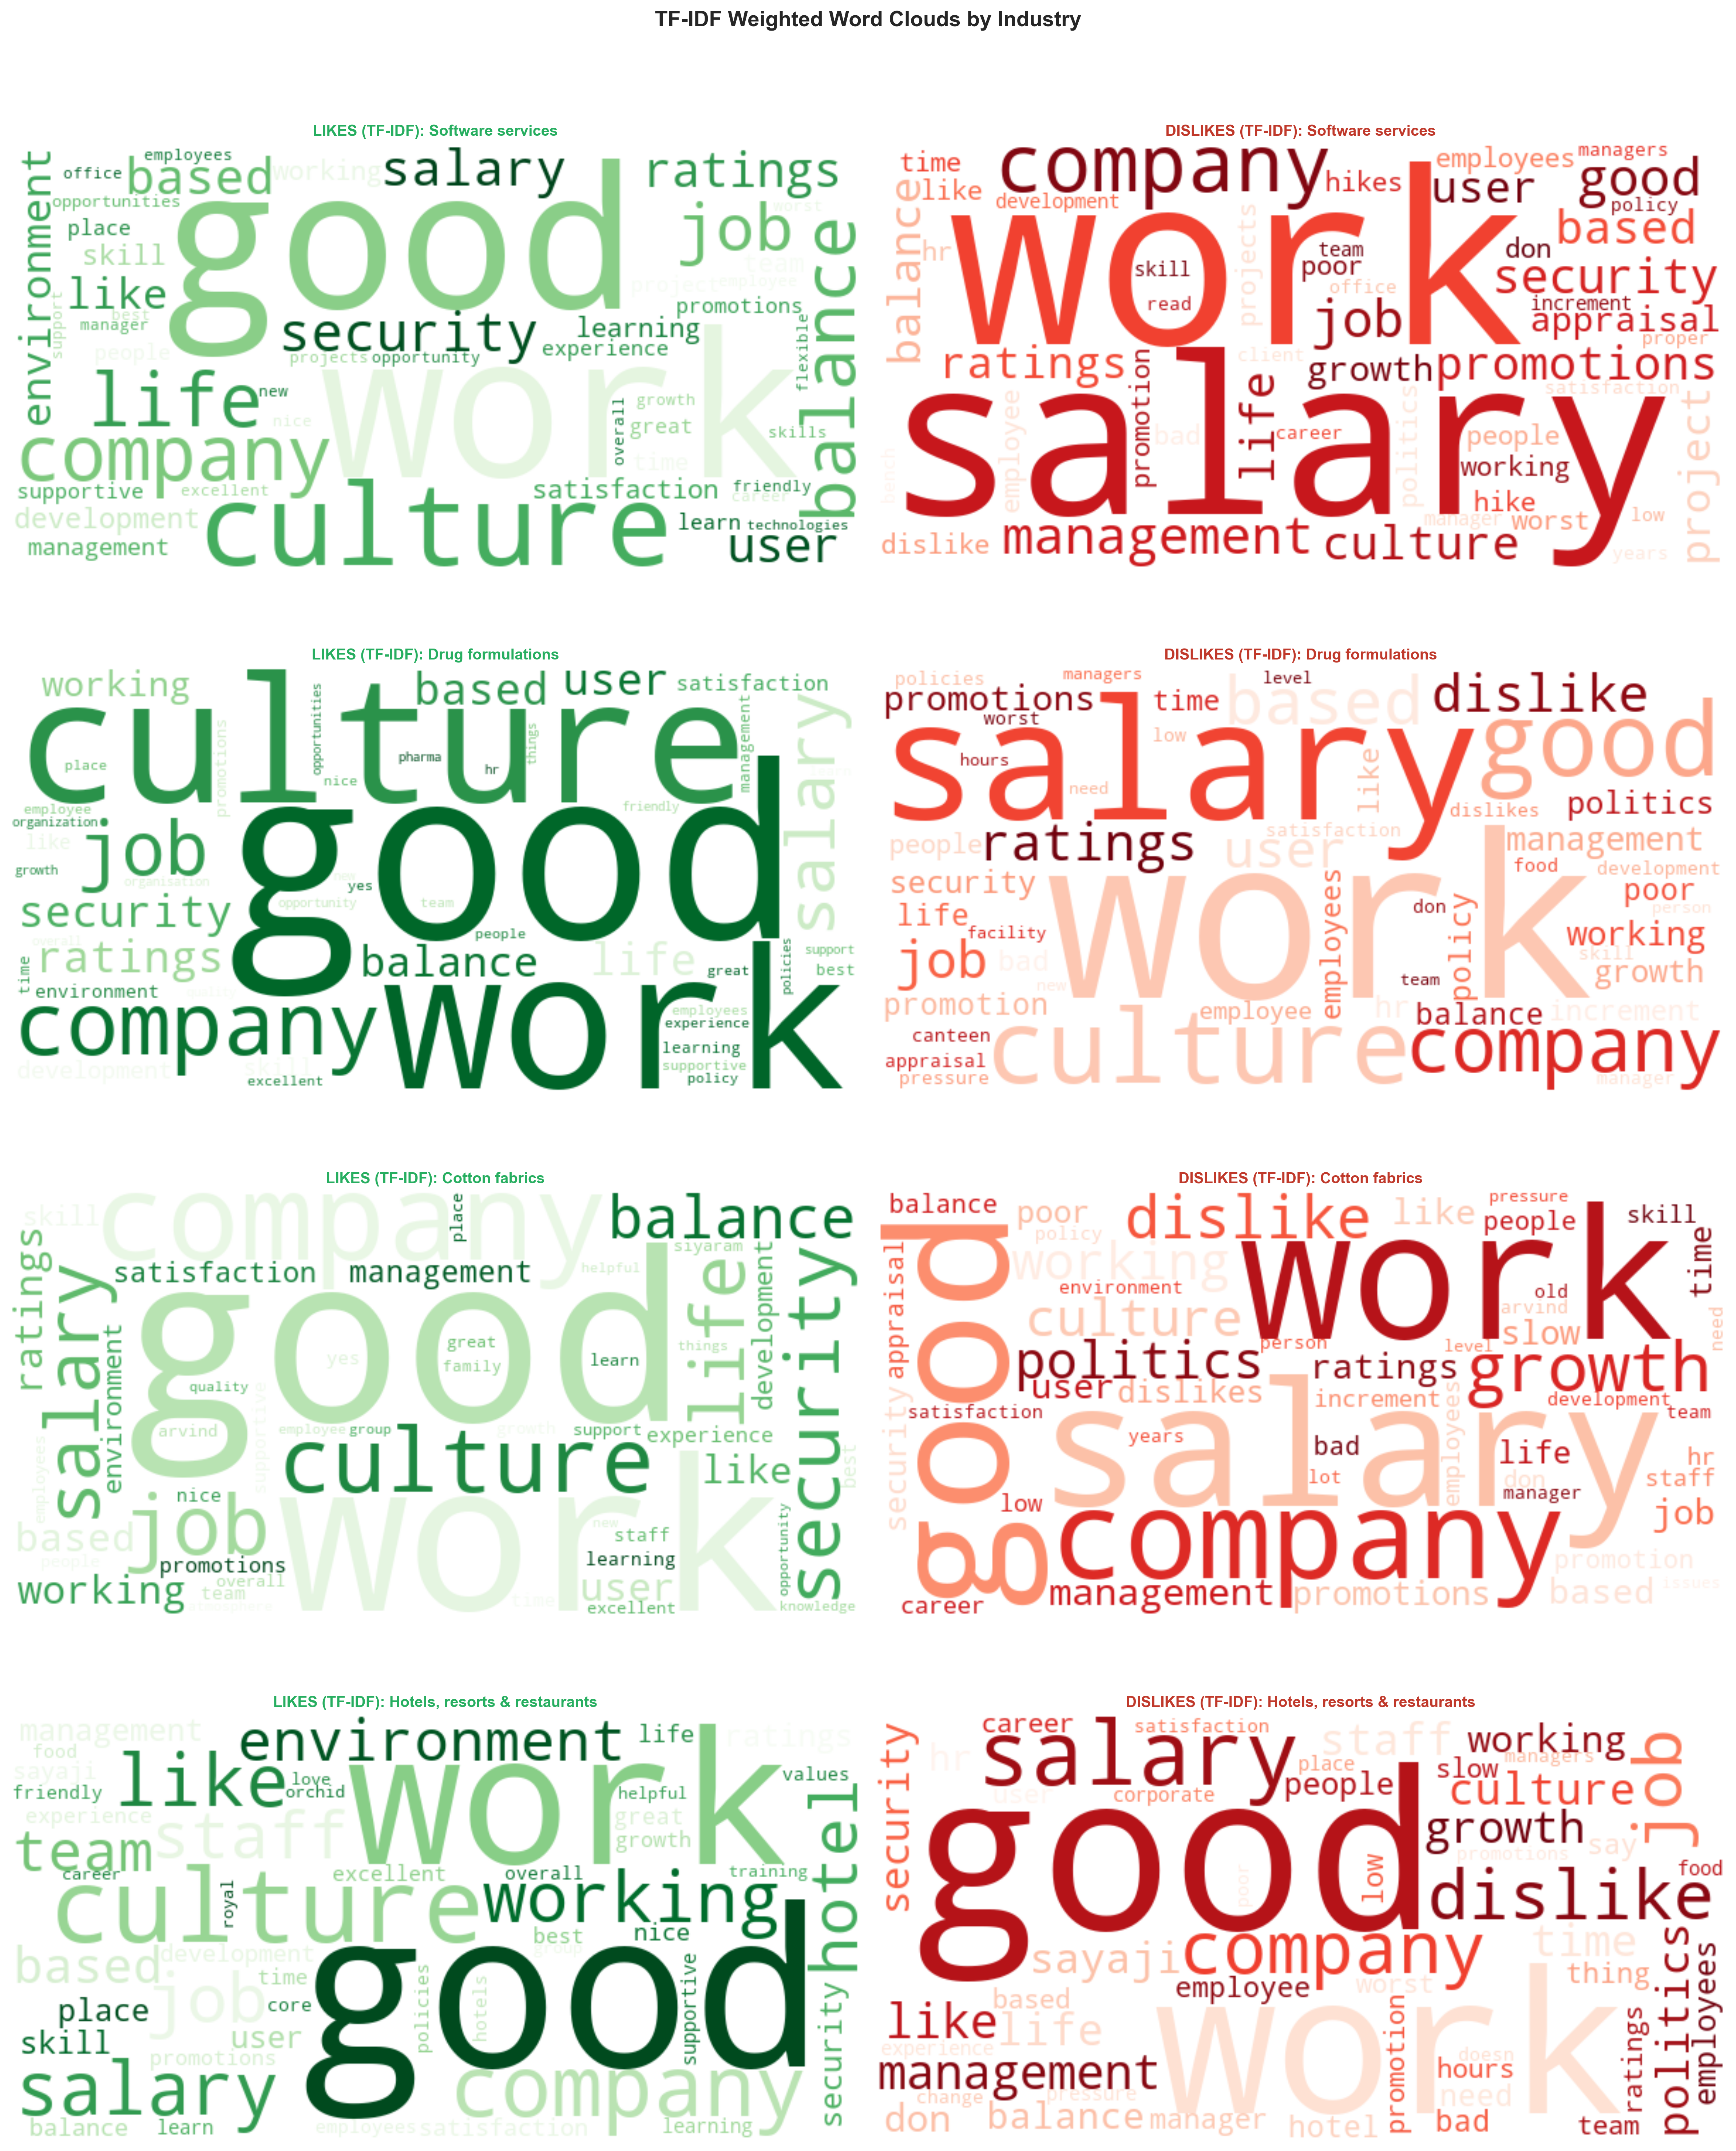
\includegraphics[width=0.95\linewidth]{industry_analysis_plots_compressed/09_tfidf_wordclouds_by_industry.jpg}
\caption{TF-IDF Weighted Word Clouds by Industry}
\label{fig:tfidf_wordclouds_industry}
\end{figure}
\section{Discussion}

\subsection{Key Insights}

\begin{enumerate}
    \item \textbf{Positive Bias}: The 3.81 mean rating suggests employees on AmbitionBox are generally satisfied, though self-selection bias likely inflates this figure.
    
    \item \textbf{Elaboration Asymmetry}: Employees write 18.6\% more for positive experiences, possibly because positive aspects are more specific while complaints tend toward general frustrations.
    
    \item \textbf{Universal Concerns}: Management quality and growth opportunities appear across companies as primary concerns regardless of industry or size.
    
    \item \textbf{Temporal Stability}: Despite platform growth, sentiment patterns remain consistent, suggesting stable workplace satisfaction trends in Indian industry.
\end{enumerate}

\subsection{Practical Applications}

The extracted features and insights enable:
\begin{itemize}
    \item Automated monitoring of company reputation
    \item Benchmarking against peer organizations
    \item Identification of improvement areas from text analysis
    \item Predictive modeling for employee satisfaction
\end{itemize}

\section{Conclusion}

We have created a complete pipeline from scraping review data for the companies provided to feature extraction that can be used for natural language processing tasks to link textual review data with company financial performance.

\begin{itemize}
    \item A robust scraping framework for AmbitionBox data
    \item Comprehensive text preprocessing for Indian English
    \item Multi-dimensional feature extraction combining sentiment, keywords, and TF-IDF
    \item Rich visualizations revealing workplace satisfaction patterns
\end{itemize}


\section*{Technical Implementation}

\textbf{Libraries Used:}
\begin{itemize}
    \item \textbf{Data Processing:} Pandas, NumPy
    \item \textbf{Visualization:} Matplotlib, Seaborn, WordCloud
    \item \textbf{NLP:} NLTK, TextBlob, scikit-learn
    \item \textbf{Web Scraping:} Selenium WebDriver
\end{itemize}




\end{document}
